% tex file for regression

\par \indent A simple and straightforward way to model the voxel time courses
is to preform linear regression. Initially, we just used the convoluted predicted
hemodyamic response (HR) using all the conditions together and each of 
conditions individually. After realizing that the HRs themselves didn't explain
enough of the BOLD ratio, attended to add features in order to reduce/ explain
the noise we observed. Additional features that we examined included a 
linear drift, a small set the fourier series, and a few principle components.

Linear regression suggests a linear relationship between an observation's response,
$y_i$ with it's features $x_i$ (a vector who's first element is $1$ and the rest are
the values the observation $i$'s features are) in the following manner:

\begin{equation}
y_i = x_i^T \beta + \epsilon_i
\end{equation}

where $\epsilon_i \sim N(0, \sigma^2)$. Moveover we assume for each observation
($i$), the $\epsilon_i$ are independent and that the true $\beta$ value is the same.
As such we can rewrite the relationship we assume is correct in a matrix form:

\begin{equation}
Y = X\beta + \epsilon
\end{equation}

This relationship requires a $X$ feature matrix, which presents each distinct feature
as a column and sees each observation get a single row to represent it's values.
Assuming $\epsilon \sim N(0,\sigma^2 I)$ isn't automatic, so we will need to check 
the validity of this assumptions, as discussed in the \textit{"Normality Assumptions"} 
section. As might be expected, we do not know the true value of $\beta$ and as such
need to estimate, using matrix algebra we get a closed from solution:

\begin{equation}
\hat{\beta} =(X^T X)^{-1} X^T 
\end{equation}

This equation does require $(X^T X)$ to be invertible, but even when it is not, we
can use the psuedo inverse, represented  $(X^T X)^{-}$ to get a non-unique value
for $\hat{\beta}$.
\par To consider the strength of the effects of these predictors, we looked 
at t-tests of the corresponding estimated coefficients for each voxel, as 
discussed under \textit{"Hypothesis Testing"}. The validity of these t-tests and 
their corresponding "p-values" is largely dependent on how good our assumptions 
of linearity and normally-distributed errors are. 

\subsubsection{More about potential features:}
\par Other than the basic HR feature/features, and a column of $1$s in our feature matrix
(to account for a ``intercept'' term/ non-zero average value), we experimented with 
include a few features for the first principle components of a of time $\times$ time 
matrix and the first few functions of the Fourier series.  As noted above these 
additional features helped account for the noise in the observed BOLD ratio 
fluxuation.

\vspace{2mm}
\textbf{Principle Components}
\vspace{2mm}
\par This matrix use to obtain the principle components was the correlation between 
each individual voxel time course with other voxel's time course ($A^TA$ where 
$A$ is a voxel $time$ time matrix). It should be noted that this matrix $A^TA$ only 
used the voxels inside the brain. ***Add Jane's Stuff about why we'd need to
use the first 6 pcs***

\vspace{2mm}
\textbf{Fourier Series}
\vspace{2mm}
\par We included 4 features related to the first few functions of the Fourier series.
The full fourier series is represent as the following:

\begin{equation}
f(x) = \frac{1}{2} \cdot a_0 + \sum_{n=1}^{\infty} a_n \cdot cos(n x) + \sum_{n=1}^{\infty} b_n \cdot  sin(n x)
\end{equation}

but since strength of Fourier series strength comes from orthogonality of the range, 
and we are looking for a function of the range $(0, \text{num of TR})$, we change it to:

\begin{equation}
f(x) = \frac{1}{2} \cdot a_0 + \sum_{n=1}^{\infty} a_n \cdot cos(\frac{n}{\text{num of TR}} x) + \sum_{n=1}^{\infty} b_n \cdot sin(\frac{n}{\text{num of TR}} x)
\end{equation}

We used $ + \sum_{n=1}^{2} a_n \cdot cos(\frac{n}{\text{num of TR}} x) + 
\sum_{n=1}^{2} b_n \cdot sin(\frac{n}{\text{num of TR}} x)$ to be 4 features to try 
to get a low order sinusoidal fluxucations.

\subsection{Model Selection}

\par In order to select the best set of features for our $X$ matrix, and also 
compare the use of a single condition feature vs each of the 3 different types
of conditions as 3 seperate features we decided to utilize model comparison, 
specificially AIC,BIC, and Adjusted $R^2$ metrics. Using small expressive
subset of the subjects ($002$,$003$, and $014$) we abused the metric's by
averaging across all voxels and people.  We visualized values in the Figures
\ref{fig:AIC},\ref{fig:BIC}, and \ref{fig:adjR2}, where the x axis follows the 
following structure in Table \ref{tab:plot}.

\par From these plots, you can observe that we don't gain my from adding
the conditions seperated, and from the BIC, we decided that the fourier
features didn't add enough benefit to justify the increase of features, so we'll
be using the model that includes a single HRF for all the conditions, a linear
drift feature, and the first 6 principle components. It is possible that this is dangerous, 
and even with these features we could have over fit beyond just the noise and into 
the territory of the hemodyamic response.

\begin{table}
\centering
	\begin{tabular}{l ||  l   |  l  |   l    | l  | l  |  l}
X value & 1 &        2       &             3       &     4         &        5        &         6       \\
	 \hline
	 & HRF &   HRF       &  HRF            & HRF         &  HRF        & HRF  \\
	 &        &   + DRIFT &  + DRIFT      & + DRIFT  &  + DRIFT   & + DRIFT  \\
	 &        &                 &  + FOURIER &  + PCA 4 &  + PCA 6   & + FOURIER \\
	 &        &                 &                      &                &                   & +  PCA 6 \\
	

	\end{tabular}
\caption{Explaining Plot X values}
\label{tab:plot}
\end{table}


%\begin{table}
%
%\begin{minipage}[b]{1\linewidth}
%	\centering
%	\scriptsize{\begin{tabular}{l ||   l  |  l  | l  | l  |l   |  l}
%	 & HRF &   HRF     &  HRF       & HRF      &  HRF       & HRF  \\
%	 &     &   + DRIFT &  + DRIFT   & + DRIFT  &  + DRIFT   & + DRIFT  \\
%	 &     &           &  + FOURIER &  + PCA 4 &  + PCA 6   & + FOURIER \\
%	 &     &           &            &          &            & +  PCA 6 \\
%	\hline
%	All conditions together   &  589.313 &  503.388 &  452.366 & 337.296 & 288.452 &   266.126 \\
%	All conditions seperately & 587.824 &  501.184 &  449.337 &   331.995 & 286.85 &   264.756 \\
%	\end{tabular}}
%	\label{tab:AIC}
%	\center{\caption{AIC}}
%\end{minipage}	
%
%\begin{minipage}[b]{1\linewidth}
%	\centering
%	\scriptsize{\begin{tabular}{l ||   l  |  l  | l  | l  |l   |  l}
%	 & HRF &   HRF     &  HRF       & HRF      &  HRF       & HRF  \\
%	 &     &   + DRIFT &  + DRIFT   & + DRIFT  &  + DRIFT   & + DRIFT  \\
%	 &     &           &  + FOURIER &  + PCA 4 &  + PCA 6   & + FOURIER \\
%	 &     &           &            &          &            & +  PCA 6 \\
%	\hline
%	All conditions together    &  596.409 &  514.032 &  477.202 &    365.68 &316.835&  308.702\\
%	All conditions seperately & 602.016 &  518.924 &  481.269  360.379 & &  322.33 & 314.427 \\
%	\end{tabular}}
%	\label{tab:BIC}
%	\caption{BIC}
%\end{minipage}	
%
%
%\begin{minipage}[b]{1\linewidth}
%	\centering
%	\scriptsize{\begin{tabular}{l ||   l  |  l  | l  | l  |l   |  l}
%	 & HRF &   HRF     &  HRF       & HRF      &  HRF       & HRF  \\
%	 &     &   + DRIFT &  + DRIFT   & + DRIFT  &  + DRIFT   & + DRIFT  \\
%	 &     &           &  + FOURIER &  + PCA 4 &  + PCA 6   & + FOURIER \\
%	 &     &           &            &          &            & +  PCA 6 \\
%	\hline
%	All conditions together    & 0.007  &  0.198  &  0.323  &  0.527   &  0.596  & 0.631 \\
%	All conditions seperately & 0.02   &  0.211  &  0.337  &    0.536  & 0.601  & 0.635\\
%	\end{tabular}}
%	\label{tab:adjR2}
%	\caption{Adjusted $R^2$}
%\end{minipage}
%
%\end{table}



\begin{figure}
\centering
	\begin{minipage}[b]{0.33\linewidth}
		\centering
		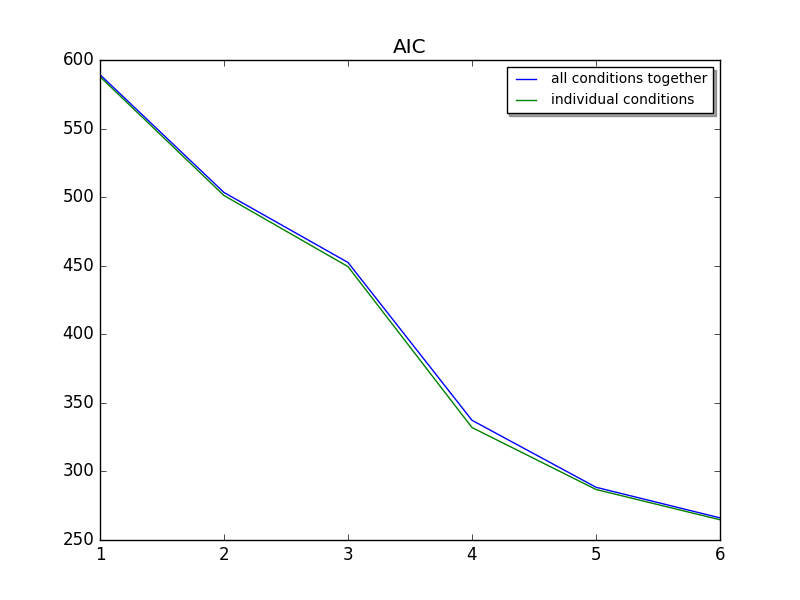
\includegraphics[width=.8\linewidth]{../images/aic_better}  

		\caption{AIC}
		\label{fig:AIC}

	\end{minipage}
	\quad
	\begin{minipage}[b]{0.33\linewidth}
		\centering
		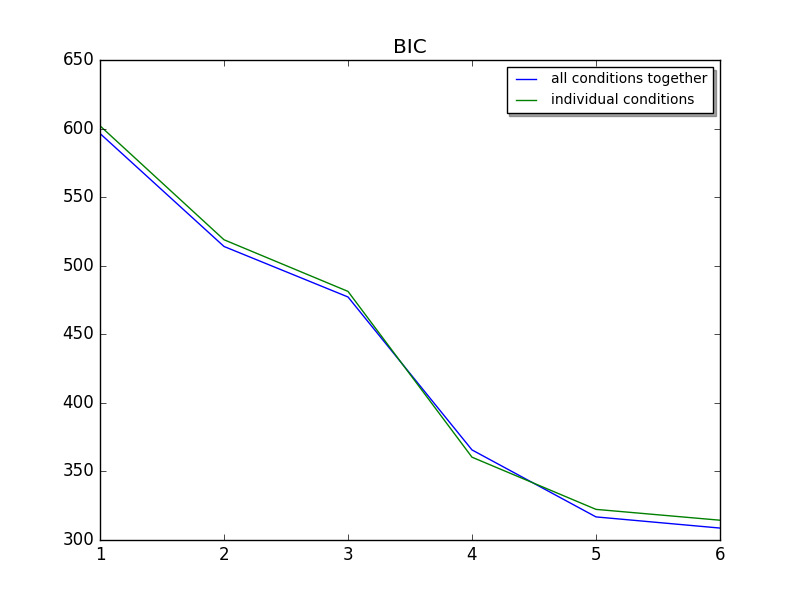
\includegraphics[width=.8\linewidth]{../images/bic_better}  
		\caption{BIC}
		\label{fig:BIC}

	\end{minipage}
		
	\begin{minipage}[b]{0.33\linewidth}
		\centering
		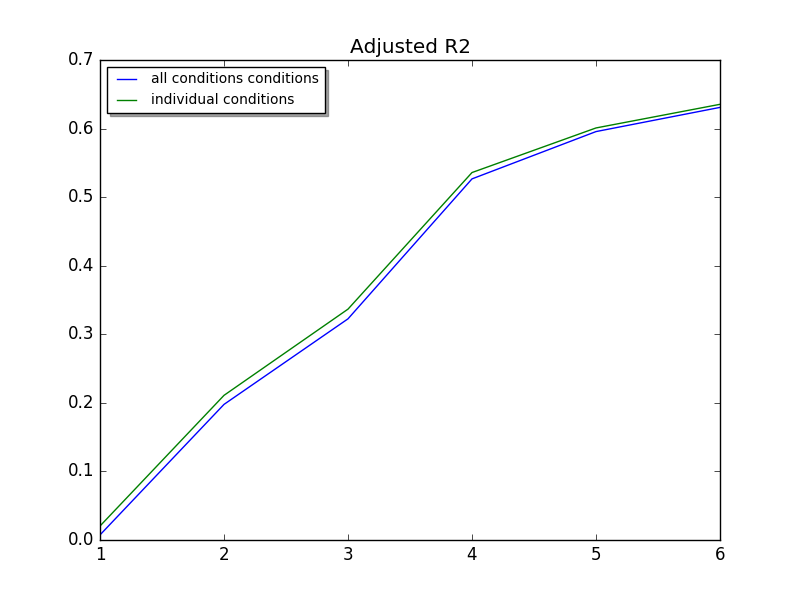
\includegraphics[width=.8\linewidth]{../images/adjr2_better}  
		\caption{Adjusted $R^2$}
		\label{fig:adjr2}

	\end{minipage}

\end{figure}

	

